\documentclass[tikz]{standalone}
\usepackage{tikz}
\usetikzlibrary{positioning, graphs}
\usetikzlibrary{graphs.standard}
\begin{document}
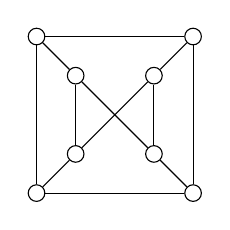
\begin{tikzpicture}
		[every node/.style={draw,circle,inner sep = 0mm, minimum size = 0.6em}]
		\graph[clockwise, radius = 4em, phase = 45, empty nodes]{subgraph C_n[n = 4, name = A]};
		\graph[clockwise, radius = 2em, phase = 45, empty nodes]{subgraph I_n[n = 4, name = B]};
		
		\foreach \i in {1, 2, 3, 4}{
			\draw (A \i) -- (B \i);
		}
		\draw (B 1) -- (B 2);
		\draw (B 2) -- (B 4);
		\draw (B 4) -- (B 3);
		\draw (B 3) -- (B 1);
\end{tikzpicture}
\end{document}